%DGraph_counter_example_delete.tex



\documentclass{standalone}
% newcommands.tex

\usepackage{amssymb, latexsym}
\usepackage{bbding} % for checkmark and xsolid
\usepackage{mathtools}

% math
\newcommand{\N}{\mathbb{N}}
\newcommand{\set}[1]{\{#1\}}
\newcommand{\bset}[1]{\big\{#1\big\}}
\newcommand{\ps}{\mathcal{P}} % for powerset
\newcommand{\emptyseq}{\emptyset} % or using <>?
\newcommand{\tuple}[1]{\langle#1\rangle} % or using (#1)?
\newcommand{\btuple}[1]{\big\langle#1\big\rangle}

\newcommand{\post}{\mathit{post}}
\newcommand{\comment}{\mathit{comment}}
\newcommand{\emptypost}{\mathit{empty}}
\newcommand{\acct}{\brown{\mathit{acct}}}

\newcommand{\yes}{\green{\Checkmark}}
\newcommand{\no}{\red{\XSolidBrush}}

\newcommand{\Key}{{\sf Key}}
\newcommand{\Val}{{\sf Val}}

\newcommand{\h}{\mathcal{H}}
%%%%%%%%%%%%%%% system models %%%%%%%%%%%%%%%
\newcommand{\E}{E}
\newcommand{\evar}{\mathit{e}}
\newcommand{\fvar}{\mathit{f}}
\newcommand{\Event}{{\sf Event}}
\newcommand{\REvent}{{\sf REvent}}
\newcommand{\WEvent}{{\sf WEvent}}
\newcommand{\HEvent}{{\sf HEvent}}
\newcommand{\op}{{\sf op}}
\newcommand{\Op}{{\sf Op}}
\newcommand{\opvar}{\mathit{op}}
\newcommand{\readevent}{{\sf R}}
\newcommand{\Read}{{\sf Read}\;}
\newcommand{\writeevent}{{\sf W}}
\newcommand{\Write}{{\sf Write}\;}
\newcommand{\WriteTx}{{\sf WriteTx}}
\newcommand{\W}{{\sf W}}
\newcommand{\R}{{\sf R}}
\newcommand{\T}{T}
%%%%%%%%%%%%%%% system models %%%%%%%%%%%%%%%

%%%%%%%%%%%%%%% axioms %%%%%%%%%%%%%%%
\renewcommand{\ae}{\mathcal{A}}
\newcommand{\axiom}{\Phi}
\newcommand{\rel}[1]{\xrightarrow{#1}}
\newcommand{\comp}{\;;\;}
\newcommand{\po}{{\sf po}}
\newcommand{\so}{\textsc{so}}
\newcommand{\rb}{\textsc{rb}}
\newcommand{\cb}{\textsc{cb}}
\newcommand{\vis}{\textsc{vis}}
\newcommand{\ar}{\textsc{ar}}
\newcommand{\hist}{\text{Hist}}
\newcommand{\intaxiom}{\textsc{Int}}
\newcommand{\extaxiom}{\textsc{Ext}}
\newcommand{\sessionaxiom}{\textsc{Session}}
\newcommand{\prefixaxiom}{\textsc{Prefix}}
\newcommand{\rbaxiom}{\textsc{ReturnBefore}}
\newcommand{\cbaxiom}{\textsc{CommitBefore}}
\newcommand{\conflict}{\bowtie}
\newcommand{\noconflictaxiom}{\textsc{NoConflict}}
\newcommand{\realtimesnapshotaxiom}{\textsc{RealtimeSnapshot}}
%%%%%%%%%%%%%%% axioms %%%%%%%%%%%%%%%

%%%%%%%%%%%%%%% consistency models %%%%%%%%%%%%%%%
\newcommand{\si}{\textsc{SI}}
\newcommand{\ansisi}{\textsc{ANSI-SI}}
\newcommand{\rtsi}{\textsc{RealtimeSI}}
\newcommand{\gsi}{\textsc{GSI}}
\newcommand{\parallelsi}{\textsc{PSI}}
\newcommand{\pcsi}{\textsc{PCSI}}
\newcommand{\strongsi}{\textsc{StrongSI}}
\newcommand{\strongsessionsi}{\textsc{SI}} % StrongSessionSI
\newcommand{\sessionsi}{\textsc{SessionSI}}
\newcommand{\nmsi}{\textsc{NMSI}}
\newcommand{\ser}{\textsc{SER}}
%%%%%%%%%%%%%%% consistency models %%%%%%%%%%%%%%%

%%%%%%%%%%%%%%% pseudo-code %%%%%%%%%%%%%%%
\newcommand{\g}{G}
\newcommand{\inducedgraph}{I}
\newcommand{\eithervar}{\mathit{either}}
\newcommand{\orvar}{\mathit{or}}
\newcommand{\reachability}{\textsc{Reachability}}
\newcommand{\reachabilityvar}{\mathit{reachability}}

\newcommand{\vertex}{\mathsf{Vertex}}
\newcommand{\edges}{\mathsf{Edge}}
\newcommand{\cons}{\mathsf{Cons}}

\newcommand{\vvar}{\mathit{v}}
\newcommand{\precvar}{\mathit{prec}}
\newcommand{\egvar}{\mathit{e}}
\newcommand{\edgevar}{\mathit{edge}}
\newcommand{\cvar}{\mathit{c}}
\newcommand{\consvar}{\mathit{cons}}

\newcommand{\BV}{\mathsf{BV}}
\newcommand{\Clause}{\mathsf{Cl}}
\newcommand{\DV}{\mathsf{DV}}
\newcommand{\formula}{\mathcal{F}}

\newcommand{\fromvar}{\mathit{from}}
\newcommand{\tovar}{\mathit{to}}
\newcommand{\typevar}{\mathit{type}}

\newcommand{\graphA}{\mathit{Dep}}
\newcommand{\graphB}{\mathit{AntiDep}}
\newcommand{\knowninducedgraph}{\mathit{KI}}
%%%%%%%%%%%%%%% pseudo-code %%%%%%%%%%%%%%%

%%%%%%%%%%%%%%% proof %%%%%%%%%%%%%%%
\newcommand{\inv}{\textsc{Inv}\;}
\newcommand{\case}{\textsc{Case}}
\newcommand{\casei}{\case\; I}
\newcommand{\caseii}{\case\; II}
%%%%%%%%%%%%%%% proof %%%%%%%%%%%%%%%

%%%%%%%%%%%%%%% checking %%%%%%%%%%%%%%%
\providecommand{\G}{}
\renewcommand{\G}{\mathcal{G}}
\renewcommand{\H}{\mathcal{H}}

\newcommand{\SO}{\textsf{SO}}
\newcommand{\WR}{\textsf{WR}}
\newcommand{\WW}{\textsf{WW}}
\newcommand{\RW}{\textsf{RW}}
%%%%%%%%%%%%%%% checking %%%%%%%%%%%%%%%

% colors
\newcommand{\red}[1]{\textcolor{red}{#1}}
\newcommand{\green}[1]{\textcolor{green}{#1}}
\newcommand{\blue}[1]{\textcolor{blue}{#1}}
\newcommand{\cyan}[1]{\textcolor{cyan}{#1}}
\newcommand{\brown}[1]{\textcolor{brown}{#1}}
\newcommand{\teal}[1]{\textcolor{teal}{#1}}
\newcommand{\purple}[1]{\textcolor{purple}{#1}}

\newcommand{\cobra}{\textsc{Cobra}}

\newcommand{\keyxvar}{\textcolor{cyan}{\mathit{x}}}
\newcommand{\keyyvar}{\textcolor{brown}{\mathit{y}}}

\usepackage{tikz}
\usetikzlibrary{shapes, positioning, arrows.meta, decorations.pathmorphing}

\begin{document}

  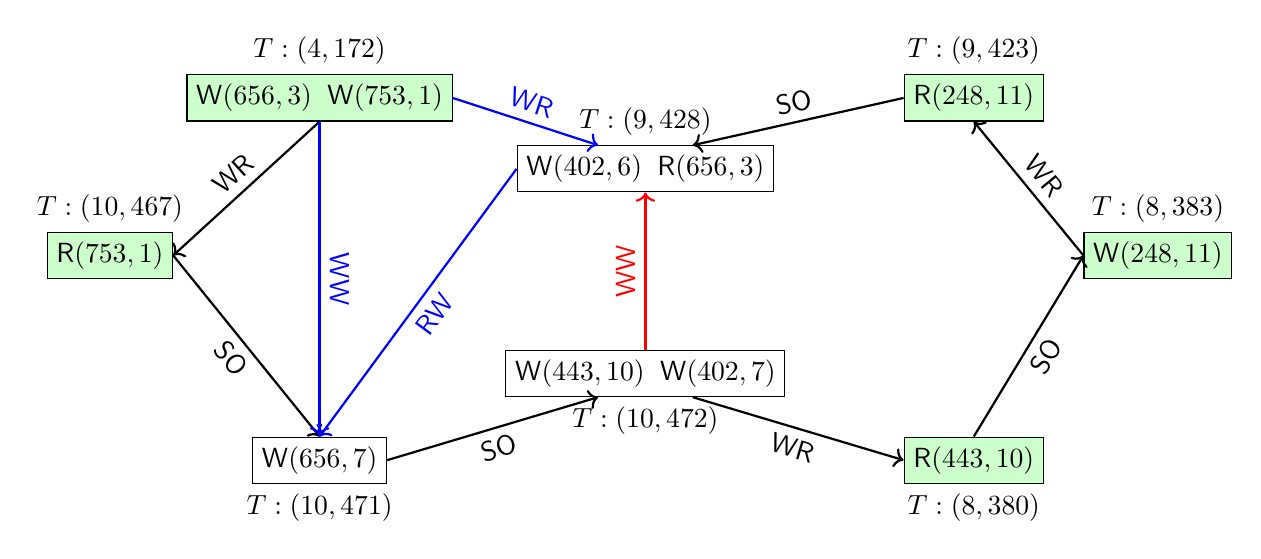
\begin{tikzpicture}[model/.style = {draw, minimum size = 15pt},  node distance = 0.5cm and 1.5cm]
        \node[model, label = below : {$\T: (10, 472)$}] (10472) {$\writeevent(443,10) \; \; \writeevent(402,7)$};
        
        \node[model, above = 2 cm of 10472, label = above : {$\T: (9, 428)$}] (9428) {$\writeevent(402,6) \; \; \readevent(656,3)$};

        \node[model, below left = of 10472, label = below : {$\T: (10, 471)$}] (10471) {$\writeevent(656,7)$};
        
         \node[model, above = 4 cm of 10471, label = above : {$\T: (4, 172)$}, fill=green!20] (4172) {$\writeevent(656,3) \; \; \writeevent(753,1)$};
        
        \node[model, above left = 2 cm and 1 cm of 10471, label = above : {$\T: (10, 467)$}, fill=green!20] (10467) {$\readevent(753,1)$};
        
       

        \node[model, below right =of 10472, label = below : {$\T: (8, 380)$}, fill=green!20] (8380)  {$\readevent(443,10)$};

        \node[model, above right = 2 cm and 0.5 cm of 8380, label = above : {$\T: (8, 383)$}, fill=green!20] (8383)  {$\writeevent(248,11)$};

        \node[model, above = 4 cm of 8380, label = above : {$\T: (9, 423)$}, fill=green!20] (9423)  {$\readevent(248,11)$};


        
        \path[->, thick, red, sloped] (10472.north) edge node[above] {$\WW$} (9428.south); 
        \path[->, thick, blue, sloped] (9428.west) edge node[below] {$\RW$} (10471.north); 
        \path[->, thick, sloped] (10471.east) edge node[below] {$\SO$} ([xshift=-6mm]10472.south); 
        \path[->, thick, blue, sloped] (4172.east) edge node[above] {$\WR$} ([xshift=-6mm]9428.north) ; 
        \path[->, thick, sloped] (4172.south) edge node[above] {$\WR$} (10467.east); 
        \path[->, thick, sloped] (10467.east) edge node[below] {$\SO$} (10471.north); 
        \path[->, thick, sloped] ([xshift=6mm]10472.south) edge node[below] {$\WR$} (8380.west); 
        \path[->, thick, sloped] (8380.north) edge node[below] {$\SO$} (8383.west); 
        \path[->, thick, sloped] (8383.west) edge node[above] {$\WR$} (9423.south);
        \path[->, thick, sloped] (9423.west) edge node[above] {$\SO$} ([xshift=6mm]9428.north);
        
        \path[->, thick, blue, sloped] (4172.south) edge node[above] {$\WW$} (10471.north) ; 
        %\path[dashed, ->, thick, purple, sloped] (10471.north)  edge [out=100,in=-100] node[above] {$\WW$}  (4172.south) ; 
        %\path[dashed, -latex, color=orange] (9428.south)  edge [out=-70,in=70] node[right] {$\WW$}  (10472.north) ;
    \end{tikzpicture}

\end{document}